\chapter{Software Parallelisability Metrics}
\label{metrics}
\qquad This chapter defines proposed software source code parallelizability metrics and gives the basic intuition behind them. It was decided, that all parallelizability metrics would be computed on the Program Dependence Graph (PDG) intermediate representation of programs (see \ref{background-program-dependence-graph}) and would rely on dependence analysis theory (see \ref{background-dependence-theory}) as their foundation.\newline
\null\qquad The chapter is structured in the following way. Section \ref{metrics-foundation-and-perspective} puts the metrics work into the context and gives the general perspective from which one has to look at parallelisability metrics. Section \ref{metrics-use} gives a motivating example and presents the output, devised metrics should ideally provide. Section \ref{metrics-metric-groups} introduces the actual metrics, along with the basic motivation for them. Metrics are introduced as a set of conceptual groups. Each group has roughly the same intuition and motivation for all its metrics.

\section{General foundation and perspective of the work} \label{metrics-foundation-and-perspective}

\subsection{Diversity in modern computer languages}
\label{metrics-diversity-in-modern-computer-languages}
\qquad There are thousands of different languages in the modern field of computer science. Computer programming languages have passed a long way from assembly languages operating at the level of native machine instructions to languages operating with concepts at a much higher abstraction levels. The reason behind such a change in the domain of computer languages is the ease, with which a human programmer can write a software.\newline
\null\qquad Unfortunately, this move to a higher-level languages comes with drawbacks as well. With the gain in programmer's productivity, such change also brings losses in software performance. It becomes increasingly difficult for the compiler to translate abstract languages into the sequence of machine instructions effectively.\newline
\null\qquad If we are to use these easy for human comprehension high-level languages, we must have tools for their efficient transformation into the form, suitable for direct execution on different native machine platforms.

\subsection{The modern role of compilers}
\label{metrics-modern-role-of-compilers}
\quad As was outlined in the previous section \ref{metrics-diversity-in-modern-computer-languages}, novadays compilers perform enabling role for the use of different sorts of modern computer languages. \newline
\null\quad In the modern state of the field, the principal role of compiler is to map high-level algorithms onto different sorts of high-performance architectures. The notion of high-performance architectures is really general and usually represents the combining term for all of the following: parallel cluster, multi-core and multi-processor architectures, vector processors, pipelined superscalar processors and all the possible combinations and co-designs of these (see \cite{patterson-and-hennessy-cod} and \cite{patterson-and-hennessy-quantitative-approach}).\newline
\null\quad Before this mapping can be done, compilers must perform extensive analyses to determine what parts of program computations depend on one another and what parts can be scheduled for parallel execution on high-performance machines. These analyses are mostly dependence-based by their nature.   

\subsection{The famous 80/20 rule}
\label{metrics-famous-80-20-rule}
\qquad As in many areas, computer science has its own 80/20 rule: 20\% of the code executes 80\% of the time. The hotspots of software programs are loops and other structures of repeted computation. Hence, loops and arrays present the most fertile ground for compiler optimizations. Metrics, being considered in this work operate on loops. For every single loop PPar tool (see chapter \ref{ppar-tool}) computes a vector of metrics (features), characterizing it. Parallelizability metrics can be devised for the whole program functions or fragments of code, but for the start, loops seem to be the most interesting and promising program parts. 

\subsection{Dependence-based approach to metrics computation}
\label{metrics-dependence-based-approach}
\qquad Compiler parallelisation of program statements is basically hindered by the execution-order constraints imposed on those statements, which, in turn, are defined by different sorts of program dependencies, which were described in the section \ref{background-dependence-theory} of the thesis. That consideration makes it clear, that in order to be credible software parallelizability metrics must be based on loop dependence properties and constraints. Program Dependence Graph (PDG) (see \ref{background-program-dependence-graph}) represents an intermediate representation of the program, which reflects all types of dependencies present in the program. 

\section{Metrics use}
\label{metrics-use}
\qquad The main goal of software parallelizability metrics is to provide a developer with additional feedback regarding loop parallelizability, which could extend binary "yes"/"no" answers of modern parallelizing compilers (see section \ref{background-modern-parallelisability-advisor-tools}) by providing some quantitative measures of loop algorithmic parallelizability. Not only compiler answers have a binary nature, as it is shown in the sections \ref{background-modern-parallelisability-advisor-tools} and \ref{analysis-manual-analysis}, sometimes Intel compiler has to be over-conservative and assumes presence of dependencies, where they do not actually exist. Such feedback might be misleading for inexperienced parallel software developer.\newline   
\null\qquad Ideally, metrics should provide a quantitative measure of loop's algorithmic parallelizability (say, this loop is 80\% parallelizible), and where compiler has to be over-conservative due to functional semantic requirements, feedback metrics do not have any constraints.\newline
\null\qquad Let's consider several little hand-written examples.  
\begin{lstlisting}[caption={Example of parallelizible loop. Intel compiler successfully parallelizes it.}, captionpos=b, label=lst:metrics-loop-motivation-0]
for (unsigned int i = 0; i < size; i++) {
	c[i] = a[i] + b[i];
}
\end{lstlisting}
\begin{lstlisting}[caption={Loop with true and anti cross iteration dependencies. Intel compiler detects dependency and refuses to parallelize the loop.}, captionpos=b, label=lst:metrics-loop-motivation-1]
for (unsigned int i = 1; i < 100; i++) {
	a[i] = a[i-1];
}
\end{lstlisting}
\null\qquad Listings \ref{lst:metrics-loop-motivation-0} and \ref{lst:metrics-loop-motivation-1} demonstrate two loops. While loop in listing \ref{lst:metrics-loop-motivation-0} is parallelizible, loop in listing \ref{lst:metrics-loop-motivation-1} is not. PPar tool (see \ref{ppar-tool}) is going to compute the following metric numbers for these loops.\newline
\null\qquad Loop in listing \ref{lst:metrics-loop-motivation-0}: \textit{loop-absolute-size}: 21, \textit{loop-payload-fraction}: 0.5714, \textit{loop-proper-sccs-number}: 0, \textit{loop-critical-payload-fraction}: 0.0000,
\textit{iterator-payload-total-cohesion}: 0.3191,
\textit{iterator-payload-non-cf-cohesion}: 0.0638.\newline 
\null\qquad Loop in listing \ref{lst:metrics-loop-motivation-1}: \textit{loop-absolute-size}: 17, \textit{loop-payload-fraction}: 0.5294, \textit{loop-proper-sccs-number}: 1, \textit{loop-critical-payload-fraction}: 0.2222,
\textit{iterator-payload-total-cohesion}: 0.2821,
\textit{iterator-payload-non-cf-cohesion}: 0.0513.\newline
\null\qquad As will be shown in the section \ref{analysis-data-interpretation-and-visualization}, metrics \textit{loop-payload-fraction}, \textit{loop-critical-payload-fraction}, \textit{iterator-payload-total-cohesion}, \textit{iterator-payload-non-cf-cohesion} correlate with loop parallelizability property the most. Metrics \textit{loop-proper-sccs-number} and \textit{loop-critical-payload-fraction} represent the critical part of the loop payload. The bigger that part and correspondingly these metrics, the harder that loop is to parallelize. Figure \ref{metrics-use-pdg-0} shows visualization of PDG for loop in listing \ref{lst:metrics-loop-motivation-1}. It is visible, that this loop has two SCCs. One for iterator (with no incoming dependencies) and the other one is for critical payload. Critical SCC contains back edge, which forms a cycle and thus SCC. This cycle represents actual dependencies between load \textit{a[i-1]} and store \textit{a[i]} in the payload, which hinder loop parallelization.\newline
\begin{figure}[htb]
\centering
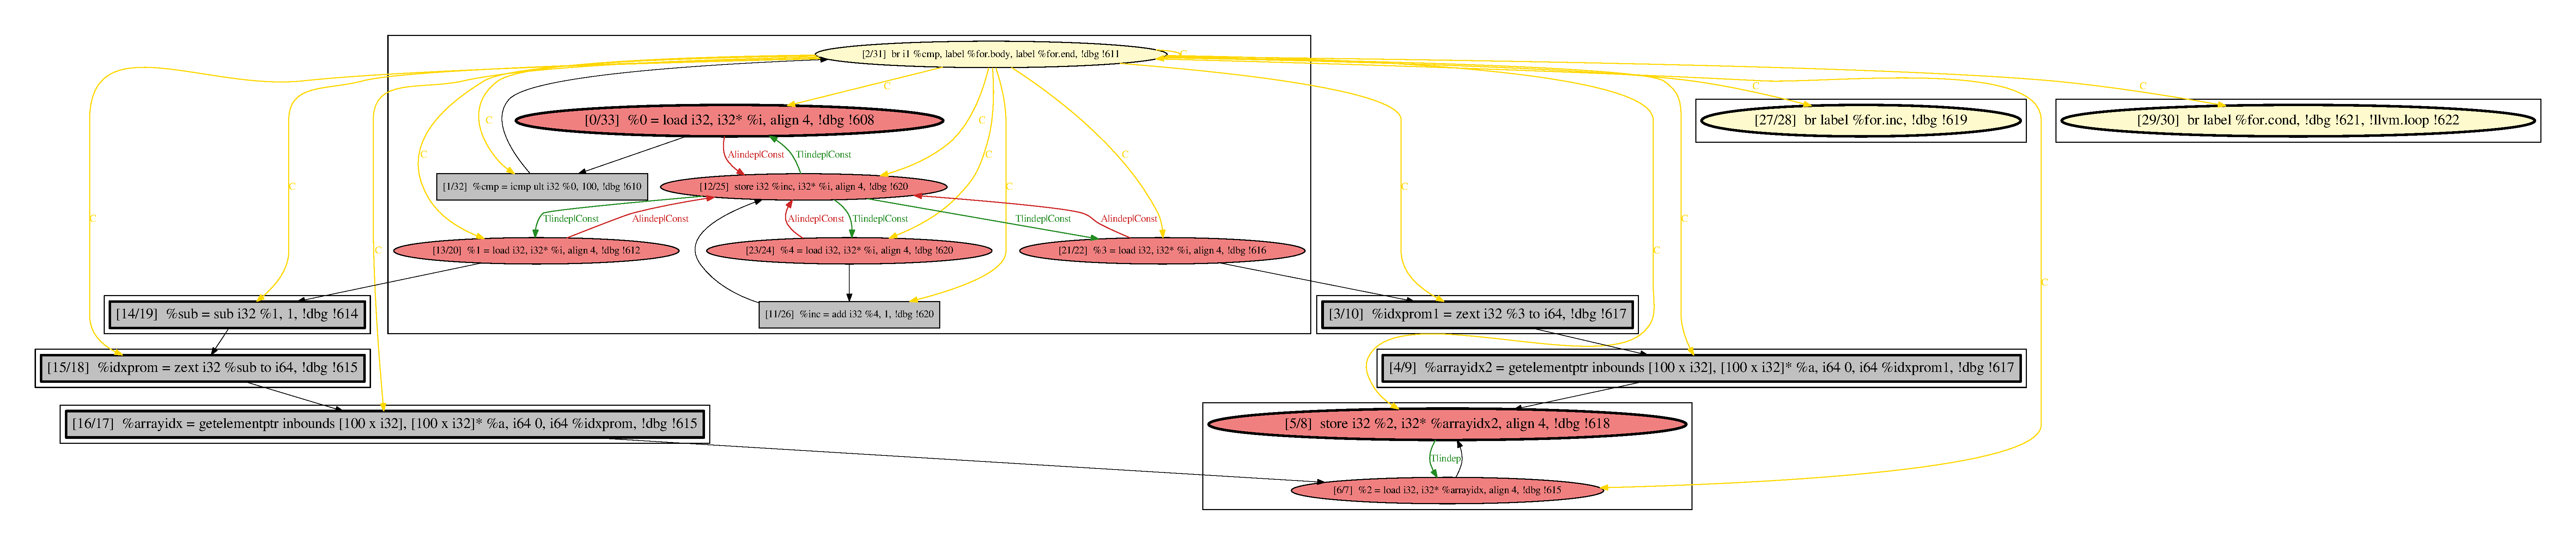
\includegraphics[width=\linewidth]{figs/metrics-use-pdg-0.pdf}
\caption{PDG of loop in listing \ref{lst:metrics-loop-motivation-0}. Graph contains two SCCs: one for iterator and one for critical payload part.}
\label{metrics-use-pdg-0}
\end{figure}
\null\qquad While loop iterator-payload cohesion metrics do not have that apparent intuition, as section \ref{analysis-data-interpretation-and-visualization} shows, they also tend to correlate with parallelizability. The bigger their values, the better the chances of loop parallelization. There are different special cases, but these two loops prove such relations between metric values and loop parallelizability.\newline
\null\qquad Let's consider another example. Loop in listing \ref{lst:metrics-loop-motivation-2} represents a loop, which performs reduction. This algorithm is parallelizible by its nature, but a programmer hid all that parallelism behind unsuccessful data structure choice (linked list). While loop in listing \ref{lst:metrics-loop-motivation-1} can be parallelized with additional memory buffer (probably cyclic shift instructions won't help because the memory area to shift might be a way larger than a processor register), loop in listing \ref{lst:metrics-loop-motivation-2} is chasing pointer and nothing can help to that code version. So, ideally, metric values for loop \ref{lst:metrics-loop-motivation-2} should be worse that those for loop \ref{lst:metrics-loop-motivation-1}. While Intel compiler won't parallelize both, metric values should show a certain difference to a programmer (say \ref{lst:metrics-loop-motivation-2} is 0\% parallelizible, \ref{lst:metrics-loop-motivation-1} is 60\% parallelizible, while \ref{lst:metrics-loop-motivation-0} is 100\% parallelizible).\newline
\null\qquad Loop in listing \ref{lst:metrics-loop-motivation-2} can be rewritten like loop in listing \ref{lst:metrics-loop-motivation-2}. That transformation immedeately lets Intel compiler to parallelize that reduction. While, Intel compiler does not do that transformation automatically, software engineer (given metric values and feedback hints) can.   
\begin{lstlisting}[caption={Algorithmic reduction, hidden behind unsuccessful data structure choice (linked-list). If linear array was used instead, the loop would be parallelized by Intel compiler. Intel compiler reports: "not a parallel candidate" for that version}, captionpos=b, label=lst:metrics-loop-motivation-2]
while (list_it != nullptr) {
	sum += list_it->value;
    list_it = list_it->next;
}
\end{lstlisting}
\begin{lstlisting}[caption={Loop with optimal data structure choice for algorithmic reduction. Intel compiler successfully parallelizes it.}, captionpos=b, label=lst:metrics-loop-motivation-3]
while (i < size) {
	sum += c[i++];
}
\end{lstlisting}
\null\qquad Metric values for these two \ref{lst:metrics-loop-motivation-2} and \ref{lst:metrics-loop-motivation-3} loops follow.\newline
\null\qquad Loop in listing \ref{lst:metrics-loop-motivation-2}: \textit{loop-absolute-size}: 14, \textit{loop-payload-fraction}: 0.4286, \textit{loop-proper-sccs-number}: 1, \textit{loop-critical-payload-fraction}: 0.5,
\textit{iterator-payload-total-cohesion}: 0.2188,
\textit{iterator-payload-non-cf-cohesion}: 0.0312.\newline
\null\qquad Loop in listing \ref{lst:metrics-loop-motivation-3}: \textit{loop-absolute-size}: 13, \textit{loop-payload-fraction}: 0.5385, \textit{loop-proper-sccs-number}: 1, \textit{loop-critical-payload-fraction}: 0.4286,
\textit{iterator-payload-total-cohesion}: 0.2759,
\textit{iterator-payload-non-cf-cohesion}: 0.0345.\newline
\null\qquad Metric \textit{loop-critical-payload-fraction} exibit such idealistically expected pattern for this particular case. Metrics \textit{iterator-payload-total-cohesion}, \textit{iterator-payload-non-cf-cohesion} do that as well, but in order to reach ideally expected feedback (if it is principally possible), some tuning and possibly even additional metrics and modifications of these, are still required.

\section{Metric Groups}
\label{metrics-metric-groups}
\qquad The whole set of proposed metrics is divided into several conceptual groups. To provide an illustrative description of different metrics, let's consider a loop \ref{lst:metrics-loop-example} given below. This loop is taken form EP NAS benchmark (see \ref{benchmarks}).
\begin{lstlisting}[caption={Example loop, taken from EP NAS benchmark}, captionpos=b, label=lst:metrics-loop-example]
for (i = 0; i < NQ; i++) {
	gc = gc + q[i];
}
\end{lstlisting}
\begin{figure}[htb]
	\centering
	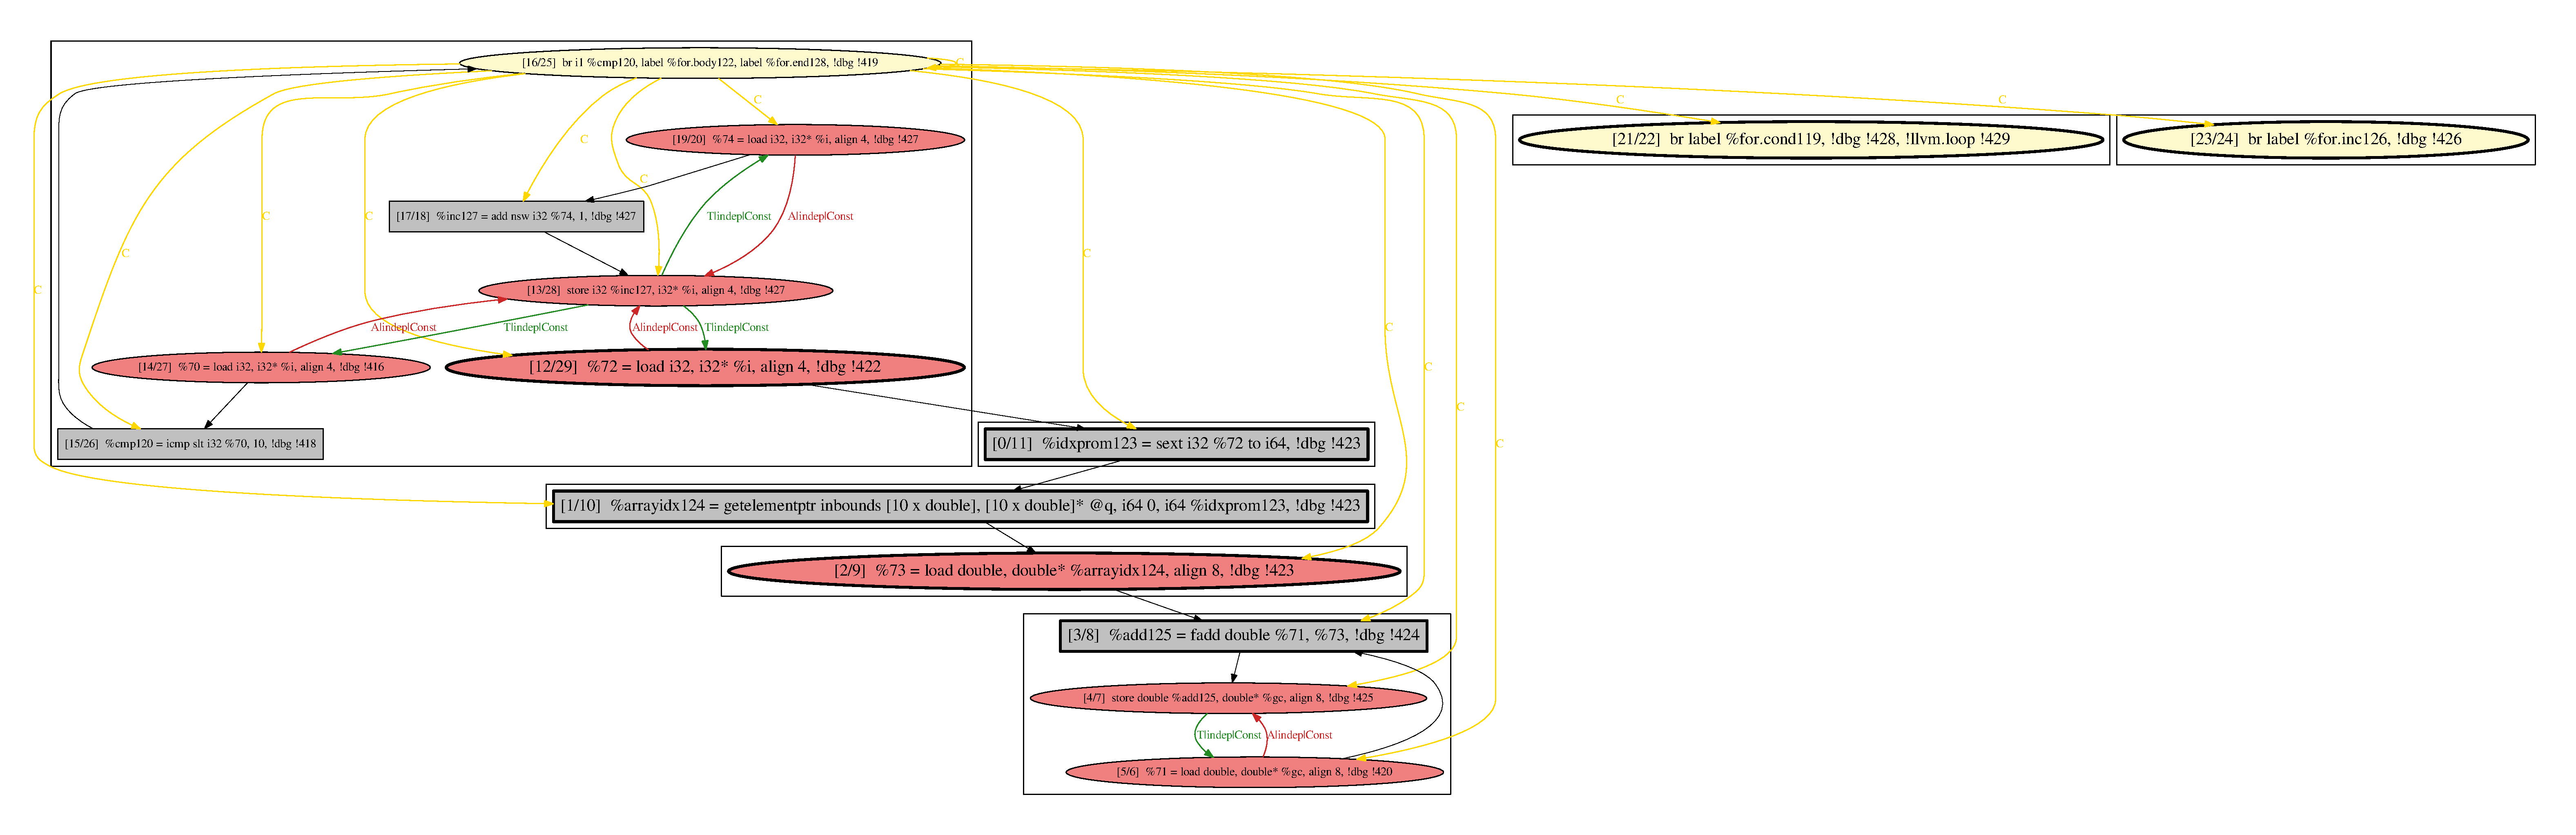
\includegraphics[width=\linewidth]{figs/metrics-example-loop-pdg.pdf}
	\caption{Program dependence graph (PDG) of the loop \ref{lst:metrics-loop-example}, as built and visualized by the PPar tool \ref{ppar-tool}.}
	\label{metrics-loop-example-pdg}
\end{figure}
\null\qquad Figure \ref{metrics-loop-example-pdg} above shows program dependence graph of the loop, given in the example. 

\subsection{Loop Proportion Metrics}
\label{metrics-loop-proportion-metrics}
\qquad The first group of metrics computes proportions of the loop. Like Halsted's software science metrics (see \ref{background-software-metrics-in-cs}), it draws an analogy with physical properties of objects (like size, volume, length, etc). This computation happens after PPar tool decouples a loop into iterator and payload code, as described in \ref{background-loop-decoupling}.  
\subsubsection{Loop Absolute Size}
\label{metrics-loop-absolute-size}
\qquad This metric represents the total amount of LLVM IR instructions in the loop. The intuition behind this metric is pretty staighforward: the bigger the loop, the harder it is to parallelize it. The metric has obvious drawbacks. The size of the loop does not, generally speaking, always correlates with loop parallelizability. However, it might be interesting to see, how loop absolute size correlates with loop parallelisability statistically. From figure \ref{metrics-loop-example-pdg} it is visible that the value of the metiric for the given loop \ref{lst:metrics-loop-example} is 15.
\subsubsection{Loop Payload Fraction}
\label{metrics-loop-payload-fraction}
\qquad This metric is complementary to loop absolute size metric and reflects the proportion in which iterator and payload divide the whole loop. There are different considerations behind this metric. For example, if the payload is too small relative to the size of the loop and does not perform significant amount of computations, then parallelization of this loop might not worth the effort.   

\subsubsection{Loop Proper SCCs number}
\label{metrics-loop-proper-sccs-number}
\qquad Once we decoupled a loop into iterator and payload parts, we can split payload part even further. Both iterator and payload are represented by subgraphs in the PDG of the loop. As was described in \ref{background-loop-decoupling}, iterator instructions form a strongly connected component (SCC), which has no incoming dependencies. Payload consists of a set of SCCs. These payload components have different sizes, starting from just 1 instruction and, principally, do not have any upper size limit. If SCC of PDG belongs to the payload of a loop and consists of more than 1 instruction, we call such SCC a \textbf{\textit{proper SCC}}. Usually, such components represent a true dependency in the body of a loop, preventing a loop from parallelization. Thus, the task of parallelizing compilers is to break the edges of such \textbf{\textit{proper (critical )}} SCCs, and transform these SCCs into smaller ones (possibly just 1 instruction). \newline
\null\qquad The example loop from the listing \ref{lst:metrics-loop-example} contains one such proper (critical) SCC. There is a cross-iteration dependency in the body of this loop. The partial sum is being accumulated in the \textit{gc} variable. We can see 2 edges (corresponding to true and anti dependencies) between variable \textit{gc} load and store instructions in the PDG shown on figure \ref{metrics-loop-example-pdg}. Despite the presense of cross-iteration dependency in the loop, Intel C/C++ compiler is capable of its parallelization with reduction techniques.\newline
\null\qquad Simplier loops, like the one shown on the listing \ref{lst:metrics-loop-example-1}, do not contain any SCCs of size greater than 1 (besides iterator SCC). Once we split such loops into iterator and payload parts, all SCCs in the payload are of 1 instruction size. Figure \ref{metrics-example-loop-1-pdg} provides illustration.
  
\begin{lstlisting}[float,floatplacement=H,caption={Parallelizible loop, with no cross-iteration dependencies. Taken from EP NAS benchmark.}, captionpos=b, label=lst:metrics-loop-example-1]
for (i = 0; i < 2 * NK; i++) {
	x[i] = -1.0e99;
}
\end{lstlisting}

\begin{figure}[htb]
	\centering
	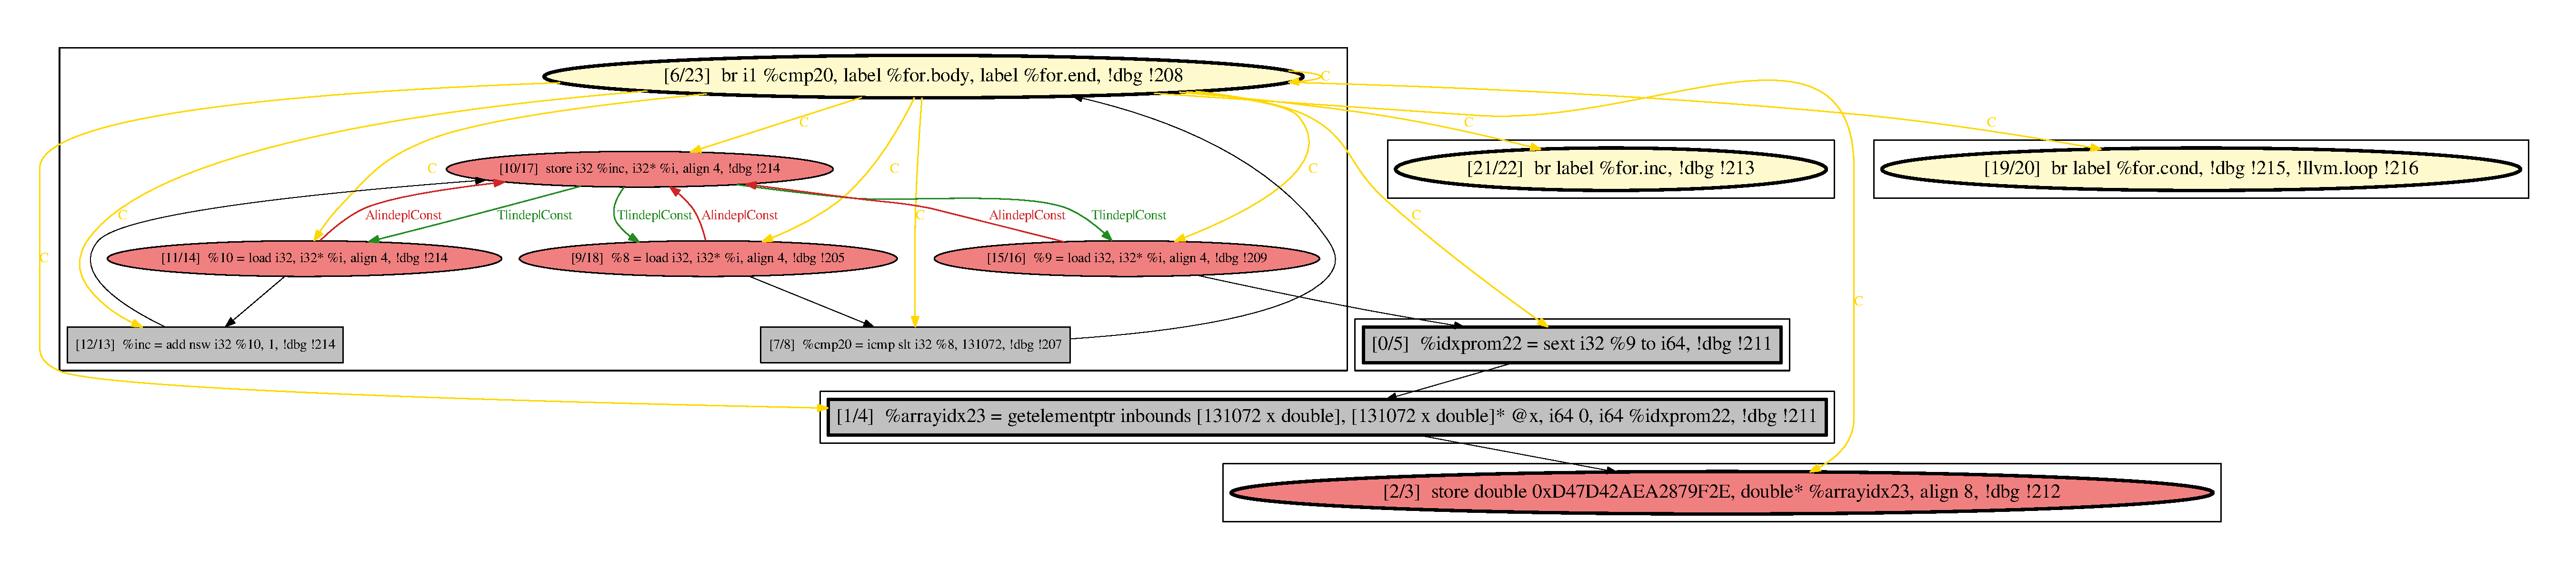
\includegraphics[width=\linewidth]{figs/metrics-example-loop-1-pdg.pdf}
	\caption{Program dependence graph (PDG) of the loop \ref{lst:metrics-loop-example-1}, as built and visualized by the PPar tool \ref{ppar-tool}.}
	\label{metrics-example-loop-1-pdg}
\end{figure}

\subsubsection{Loop Critical Payload Fraction}
\label{metrics-loop-critical-payload-fraction}
\qquad In the light of considerations given in the previous section, the fraction between critical and non-critical payload parts might have some correlation with loop parallelizability.  

\subsubsection{The problem of proper SCCs number metric}
\qquad The proper SCCs number metric was described in section \ref{metrics-loop-proper-sccs-number}. Despite the fact, that the metric seems to directly represent parallelisability inhibiting parts of the payload, ICC compiler sometimes fails to parallelise loops even with 0 metric value. Listing \ref{lst:metrics-loop-example-2} below, gives such example.
\begin{lstlisting}[float,floatplacement=H,caption={Loop, under question. Its parallelizability depends on things happening inside randlc() function. Intel compiler does not parallelize it, since it has to be conservative.}, captionpos=b, label=lst:metrics-loop-example-2]
for (i = 0; i < MK + 1; i++) {
	t2 = randlc(&t1, t1);
}
\end{lstlisting}
Figure \ref{metrics-example-loop-2-pdg} shows the PDG of the code in the listing \ref{lst:metrics-loop-example-2}. Loop \ref{lst:metrics-loop-example-2} has a simple PDG. There are no critical SCCs inside loop's payload. However, ICC compiler cannot parallelize this loop due to \textit{randlc} function call. Compiler has to be conservative and assume, that this function call introduces cross-iteration dependencies between iterations of the loop.\newline   
\begin{figure}[htb]
\centering
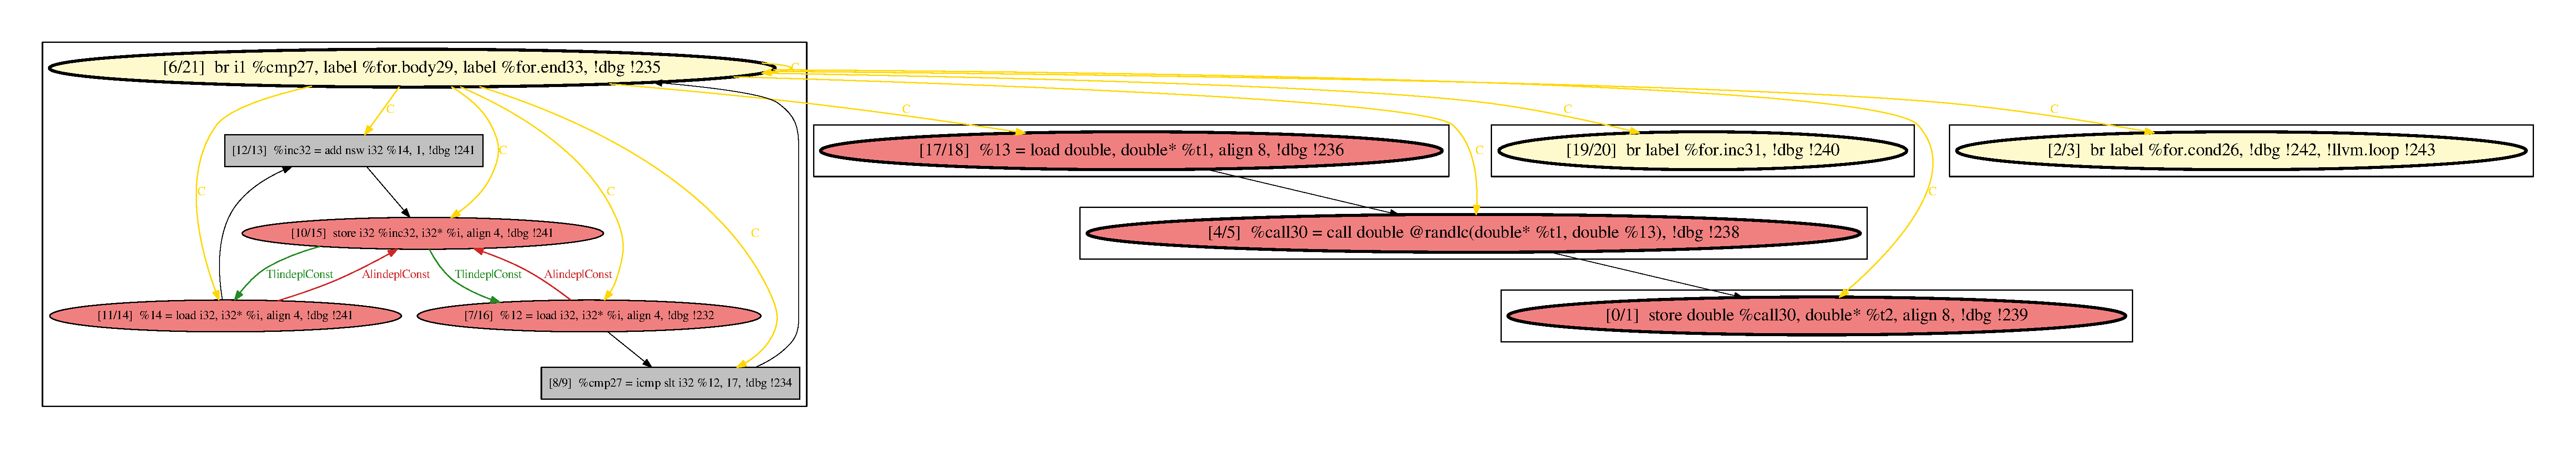
\includegraphics[width=\linewidth]{figs/metrics-example-loop-2-pdg.pdf}
\caption{Program dependence graph (PDG) of the loop \ref{lst:metrics-loop-example-2}, as built and visualized by the PPar tool \ref{ppar-tool}.}
\label{metrics-example-loop-2-pdg}
\end{figure}
\null\qquad This example exposes drawback of proper SCCs number metric. This metric only considers structural properties of PDG and does not examine the nature of instructions, constituting the loop. 

\subsection{Loop Dependence Metrics}
\label{metrics-loop-dependence-metrics}
\qquad Different types of dependencies have been described in section \ref{background-dependence-theory} of the thesis. These dependencies introduce different sorts of constraints into loops, which prevent their parallelization.\newline
\null\qquad These metrics simply count the number of dependencies in the whole loop payload, as well as in the critical part of the payload (if it is present). For payload we have: payload true dependencies number, payload anti dependencies number, payload output dependencies number and the total amount of dependencies in the payload. The same set of metric is present for the critical payload part of loops.\newline
\null\qquad The intuition behind these metrics is apparent. The bigger the amount of dependencies we have in a loop, especially in its critical part, the harder it is going to be to parallelize it.

\subsection{Loop Cohesion Metrics}
\label{metrics-loop-cohesion-metrics}
\qquad As cohesion and coupling metrics have been proposed for computer software \ref{background-cohesion-and-coupling}, these properties can also be extended in context of this work.\newline
\null\qquad These properties characterize the degree of inter-dependence between different parts of loops. In this work we introduce two main types of cohesion metrics: iterator-payload cohesion and critical payload cohesion. The first characterizes the degree of coupling between loop iterator and loop payload. The second characterizes coupling between non-critical part of loop payload (all instructions, which do not belong to proper SCCs of a loop) and payload critical part. Both of these metrics are represented as a fraction.\newline
\null\qquad Iterator-payload cohesion is defined as the ratio of a number of dependence edges between iterator and payload to the total number of edges in the whole loop (iterator and payload altogether). An edge is going from iterator to the payload, if it originates in instruction belonging to iterator SCC and ends in instruction, belonging to the payload of a loop. Edges, going in reverse direction, from loop payload to loop iterator are also counted as cohesion edges.\newline
\null\qquad Critical payload cohesion is also defined alike, as the ratio of a number of edges between critical and non-critical payload parts to the whole number of edges in a loop payload.\newline
\null\qquad Both of these cohesion metrics are further subdivided into two types: total cohesion and non-CF (non Control Flow) cohesion. Difference follows out of names. Total cohesion counts all edges, non-CF those, which are not control dependencies.\newline
\null\qquad While both of these metrics make sense, it is not that obvious, what sort of correlation we should expect.    

